%------------------------------------------------------------------------------
% CV in Latex
% Author : Charles Rambo
% Based off of: https://github.com/sb2nov/resume and Jake's Resume on Overleaf
% Most recently updated version may be found at https://github.com/fizixmastr 
% License : MIT
%------------------------------------------------------------------------------

\documentclass[A4,11pt]{article}
%\documentclass[letterpaper,11pt]{article} %For use in US
\usepackage{latexsym}
\usepackage[empty]{fullpage}
\usepackage{titlesec}
\usepackage{marvosym}
\usepackage[usenames,dvipsnames]{color}
\usepackage{verbatim}
\usepackage{enumitem}
\usepackage{hyperref}
\usepackage[english]{babel}
\usepackage{tabularx}
\usepackage{tikz}
\usepackage{xcolor}
\usepackage{url}
\usepackage{etaremune}
\renewcommand{\labelenumi}{[\theenumi]}

\hypersetup{
	colorlinks   = true,
	citecolor    = black!60,
	urlcolor     = blue
}


\begin{comment}
	I am by no means a professional when it comes to the CV's/resumes, I have
	received various trainings on how to write a CV and resume from my high 
	school, as well as the Austin College and University of Eastern Finland's
	career counseling departments. As I intend to share my CV as a template, I 
	feel that it is my responsibility to provide explanations of my work.
\end{comment}


%-----FONT OPTIONS-------------------------------------------------------------
\begin{comment}
	The font of the document will impact not just how readable it is, but how it is
	perceived. In the "The Craft of Scientific Writing" by Michael Alley, shares a
	common fonts for publication as well as their use. I have chosen to use
	Palatino for its legibility, some others are given below. There is far too much
	about typography to discus here. Note: serif fonts have short projecting
	strokes, sans-serif fonts are sans (without) these strokes.
\end{comment}


% serif
\usepackage{palatino}
% \usepackage{times} %This is the default as well
% \usepackage{charter}

% sans-serif
% \usepackage{helvet}
% \usepackage[sfdefault]{noto-sans}
% \usepackage[default]{sourcesanspro}

%-----PAGE SETUP---------------------------------------------------------------

% Adjust margins
\addtolength{\oddsidemargin}{-1cm}
\addtolength{\evensidemargin}{-1cm}
\addtolength{\textwidth}{2cm}
\addtolength{\topmargin}{-1cm}
\addtolength{\textheight}{2cm}

% Margins for US Letter size
%\addtolength{\oddsidemargin}{-0.5in}
%\addtolength{\evensidemargin}{-0.5in}
%\addtolength{\textwidth}{1in}
%\addtolength{\topmargin}{-.5in}
%\addtolength{\textheight}{1.0in}

\urlstyle{same}

\raggedbottom
\raggedright
\setlength{\tabcolsep}{0cm}

% Sections formatting
\titleformat{\section}{
	\vspace{0pt}\scshape\raggedright\large
}{}{0em}{}[\color{black}\titlerule \vspace{-1pt}]

% Ensure that .pdf is machine readable/ATS parsable
\pdfgentounicode=1

%-----CUSTOM COMMANDS FOR FORMATTING SECTIONS----------------------------------
\newcommand{\CVItem}[1]{
	\item\small{
		{#1 \vspace{-2pt}}
	}
}

\newcommand{\CVPubheading}[2]{
	\vspace{-0.5ex}\item
	\begin{tabular*}{0.97\textwidth}[t]{l@{\extracolsep{\fill}}r}
		\textbf{#1} & #2 \\
	\end{tabular*}\vspace{-1.5ex}
}

\newcommand{\CVQubheading}[3]{
	\vspace{-0.5ex}\item
	\begin{tabular*}{0.97\textwidth}[t]{l@{\extracolsep{\fill}}r}
		\textbf{#1} & #2 \\
	\end{tabular*}
   {\small #3}\vspace{-0.5ex}
}

\newcommand{\CVRubheading}[3]{
	\vspace{0.5ex}\item
	\textbf{#1}
	\begin{tabular*}{0.97\textwidth}[t]{l@{\extracolsep{\fill}}r}
		\small#2 & \small #3 \\
	\end{tabular*}\vspace{-1.55ex}
}

\newcommand{\CVSubheading}[4]{
	\vspace{-0.5ex}\item
	\begin{tabular*}{0.97\textwidth}[t]{l@{\extracolsep{\fill}}r}
		\textbf{#1} & #2 \\
		\small#3 & \small #4 \\
	\end{tabular*}\vspace{-1.5ex}
}

\newcommand{\CVTubheading}[6]{
	\vspace{-2pt}\item
	\begin{tabular*}{0.97\textwidth}[t]{l@{\extracolsep{\fill}}r}
		\textbf{#1} & #2 \\
		\small#3 & \small #4 \\
		\small#5 & \small #6 \\
	\end{tabular*}\vspace{-7pt}
}

\newcommand{\CVSubItem}[1]{\CVItem{#1}\vspace{-4pt}}

\renewcommand\labelitemii{$\vcenter{\hbox{\tiny$\bullet$}}$}

\newcommand{\CVSubHeadingListStart}{\begin{itemize}[leftmargin=0.5cm, label={}]}
%\newcommand{\resumeSubHeadingListStart}{\begin{itemize}[leftmargin=0.15in, label={}]} % Uncomment for US
\newcommand{\CVSubHeadingListEnd}{\end{itemize}}
\newcommand{\CVItemListStart}{\begin{itemize}}
\newcommand{\CVItemListEnd}{\end{itemize}\vspace{-5pt}}
	
	%------------------------------------------------------------------------------
	% CV STARTS HERE  %
	%------------------------------------------------------------------------------
	\begin{document}
		
		%-----HEADING------------------------------------------------------------------
		\begin{comment}
			In Europe it is common to include a picture of ones self in the CV. Select
			which heading appropriate for the document you are creating.
		\end{comment}
		
		\begin{minipage}[c]{0.05\textwidth}
			\-\
		\end{minipage}
		\begin{minipage}[c]{0.2\textwidth}
			\begin{tikzpicture}
				\clip (0,0) circle (1.75cm);
				\node at (0,-0.1) {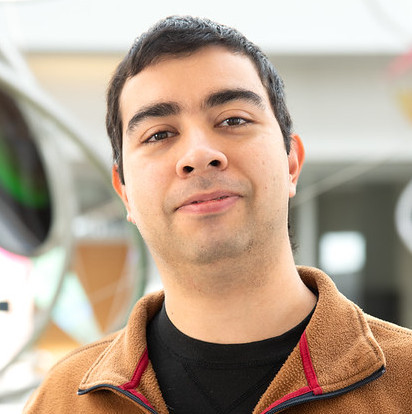
\includegraphics[width = 4cm]{53500746199_4b98a4c178_c.jpg}}; 
				% if necessary the picture may be moved by changing the at (coordinates)
				% width defines the 'zoom' of the picture
			\end{tikzpicture}
			\hfill\vline\hfill
		\end{minipage}
		\begin{minipage}[c]{0.4\textwidth}
			\textbf{\Huge \scshape{Erik Am\'ezquita}} \\ \vspace{1pt} 
			% \scshape sets small capital letters, remove if desired
			\small{+1 517-755-8202} \\
			\href{mailto:eah4d@missouri.edu}{\underline{eah4d@missouri.edu}}\\
			% Be sure to use a professional *personal* email address
			\href{https://www.linkedin.com/in/erik-amezquita/}{\underline{linkedin.com/in/erik-amezquita/}} \\
			% you should adjust you linked in profile name to be professional and recognizable
			\href{https://ejamezquita.github.io/}{\underline{ejamezquita.github.io/}}
		\end{minipage}
		\begin{minipage}[c]{0.3\textwidth}
			\vspace{1.5em}
			\small{1201 Rollins St\\371h Bond Life Sciences Center\\Columbia, MO 65211\\USA}
		\end{minipage}
		
		%-----EDUCATION----------------------------------------------------------------
		\section{Empleo y Educaci\'on}
		\CVSubHeadingListStart
		%    \CVSubheading % Example
		%      {Degree Achieved}{Years of Study}
		%      {Institution of Study}{Where it is located}
		\CVSubheading
		{{Investigador Posdoctoral $|$ \emph{\small{Biolog\'ia Vegetal (80\%) y Matem\'aticas (20\%)}}}}{Jul.~2023 -- presente}
		{Division of Plant Science \& Technology, University of Missouri}{Columbia, Missouri, EEUU}
		\CVTubheading
		{{Doctorado (PhD) $|$ \emph{\small{C\'omputo Matem\'atico Cient\'ifico e Ingenier\'ia}}}}{Ago.~2018 -- Mayo 2023}
		{Computational Mathematics, Science \& Engineering, Michigan State University}{East Lansing, Michigan, EEUU}
		{Tesis: \emph{Exploring the Mathematical Shape of Plants}}{}
		\CVTubheading
		{{Licenciatura $|$ \emph{\small{Matem\'aticas}}}}{Ago.~2013 -- Jun.~2018}
		{Departamento de Matem\'aticas, Universidad de Guanajuato}{Guanajuato, Guanajuato, M\'exico}
		{Tesis: \emph{Efficient object classification using the Euler Characteristic}}{}
		\CVSubHeadingListEnd
		
		%-----WORK EXPERIENCE----------------------------------------------------------
		\begin{comment}
			try to briefly explain what you did and why it is relevant to the position you
			are seeking
		\end{comment}
		
		\section{Proyectos desarrollados y Experiencia en Investigaci\'on Relevantes}
		\CVSubHeadingListStart
		%    \CVSubheading %Example
		%      {What you did}{When you worked there}
		%      {Who you worked for}{Where they are located}
		%      \CVItemListStart
		%        \CVItem{Why it is important to this employer}
		%      \CVItemListEnd
		\CVRubheading
		{Modelado matem\'atico de patrones y distribuciones espaciales transcritos de ARNm a nivel subcelular}
		{Division of Plant Science \& Technology, University of Missouri}{Oct.~2023 -- presente}
		\CVItemListStart
		\CVItem{Caracterizaci\'on matem\'atica de transcritos de ARNm dentro de c\'elulas de la ra\'iz de soya (\emph{Glycine max})}
		\CVItem{Uso de Python y An\'alisis Topol\'ogico de Datos para el modelado de patrones espaciales celulares}
		%\CVItem{Identificaci\'on de patrones distintivos de ARNm en c\'elulas senescentes para diversos genes}
		%\CVItem{An\'alisis desarrollado en Python con posibilidad de adaptar a m\'as datos transcript\'omicos espaciales}
		\CVItemListEnd
		\CVRubheading
		{Fenotipado autom\'atico del movimiento de \emph{Cuscuta campestris} con seguimiento de objetos}
		{Division of Plant Science \& Technology, University of Missouri}{Jul.~2023 -- Abril 2024}
		\CVItemListStart
		\CVItem{Uso de Python para detectar el movimiento de \emph{Cuscuta} a medida que \'esta se enrolla en posibles hu\'espedes}
		\CVItem{Identificaci\'on autom\'atica de tiempos y velocidades de enroscamiento dependientes de la hora del d\'ia}
		\CVItemListEnd
		\CVRubheading
		{An\'alisis matem\'atico de morfolog\'ia de nueces con tomograf\'ias 3D}
		{Division of Plant Science \& Technology, University of Missouri}{Oct.~2022 -- Dic.~2023}
		\CVItemListStart
		\CVItem{Uso de Python para analizar tomograf\'ias 3D y calcular 50 fenotipos morfol\'ogicos de nueces (\emph{Juglans regia})}
		\CVItem{Determinaci\'on de los 4 fenotipos morfol\'ogicos m\'as predictivos de caracter\'isticas de interes comercial}
		\CVItemListEnd
		\CVRubheading
		{An\'alisis de datos gen\'omicos a trav\'es de topolog\'ia algebraica aplicada}
		{Dept. of Computational Mathematics, Science \& Engineering, Michigan State University}{Ene.~2020 -- Mar.~2023}
		\CVItemListStart
		\CVItem{Reducci\'on de dimensi\'on y clusterizaci\'on de perfiles gen\'eticos de tejido pulmonar sano y cancer\'igeno}
		\CVItem{Detecci\'on de subtipos de cancer pulmonar previamente no identificados}
		\CVItemListEnd
		\CVRubheading
		{Modelado estad\'istico de la distribuci\'on de gl\'andulas de aceite en c\'itricos}
		{Dept. of Computational Mathematics, Science \& Engineering, Michigan State University}{Oct.~2021 -- Dic.~2022}
		\CVItemListStart
		\CVItem{Desarrollo de software en Python para analizar tomograf\'ias 3D de c\'itricos y aislar sus gl\'andulas de aceite}
		\CVItem{Uso de estad\'istica direccional para modelar la distribuci\'on de las gl\'andulas a lo largo de la c\'ascara de la fruta}
		\CVItemListEnd
		\CVRubheading
		{Caracterizaci\'on matem\'atica de la morfolog\'ia de granos de cebada}
		{Dept. of Computational Mathematics, Science \& Engineering, Michigan State University}{Ago.~2019 -- Dic.~2021}
		\CVItemListStart
		\CVItem{Desarrollo de software en Python para analiza tomograf\'ias 3D de espigas de cebada (\emph{Hordeum vulgare})}
		\CVItem{Uso de aprendizaje de m\'aquina (ML) para predecir el genotipo de la semilla basado solo en su morfolog\'ia}
		\CVItemListEnd
		\CVSubHeadingListEnd
		
		\section{Habilidades generales}
		\begin{itemize}[leftmargin=0.5cm, label={}]
			\small{\item{
					\textbf{Idiomas}{: Espa\~nol (nativo), Ingl\'es (pr\'acticamente nativo), Franc\'es (elemental)} \\
					\textbf{Programaci\'on}{: Python (NumPy, SciPy, Pandas, Scikit-Learn, Scikit-Image), R (tidyverse), C/C++, bash/unix} \\
					\textbf{Tecnolog\'ias}{: \LaTeX, RMarkdown, Jupyter, vim, html/css} \\
			}}
		\end{itemize}
		
		%-----HONORS AND AWARDS--------------------------------------------------------
		\section{Experiencia Docente}
		\CVSubHeadingListStart
		%    \CVSubheading %Example
		%      {What}{When}
		%      {Short Description}{}
		\CVSubheading
		{Docente titular}{Ene.~2025 -- presente}
		{Division of Plant Science \& Technology, University of Missouri}{}
		\CVItemListStart
		\CVItem{PLNT\_SCI 2500: Introducci\'on a Python y Ciencia de Datos para Ciencias de la Vida I}
		\CVItemListEnd
		\CVPubheading{Tutor y facilitador de talleres}{Jun.~2017 -- Jun.~2021}
		\CVItemListStart
		\CVItem{\hyperref{https://sgi.mit.edu/}{}{}{SGI}. Summer Geometry Institute. Massachusets Institute of Technology. Virtual. Verano 2021}
		\CVItem{\hyperref{https://codeinplace.stanford.edu/}{}{}{Code in Place}. Stanford University. Virtual. Verano 2021}
		\CVItem{\hyperref{https://tallerdecalculo2017.eventos.cimat.mx/}{}{}{XIV Taller de Soluci\'on de Problemas de C\'alculo}. CIMAT, Guanajuato, Gto., M\'exico. Virtual. Verano 2017}
		\CVItemListEnd
		\CVSubheading
		{Auxiliar de c\'atedra}{Ago.~2019 -- Dic.~2019}
		{Dept. of Computational Mathematics, Science \& Engineering, Michigan State University}{}
		\CVItemListStart
		\CVItem{\hyperref{https://msu-cmse-courses.github.io/cmse201-S24-jb/Course_Materials-201/Syllabus/syllabus.html}{}{}{CMSE 201}: Modelado computacional y An\'alisis de Datos I}
		\CVItemListEnd
		\CVSubheading
		{Auxiliar de c\'atedra}{Ene.~2017 -- Mayo~2018}
		{Departamento de Matem\'aticas, Universidad de Guanajuato}{}
		\CVItemListStart
		\CVItem{Prec\'alculo y geometr\'ia anal\'itica. Primavera 2018}
		\CVItem{Topolog\'ia I. Oto\~no 2017}
		\CVItem{Introducci\'on a Programaci\'on en C/C++ y estructuras de datos. Verano 2017}
		\CVItem{Introducci\'on a Probabilidad. Primavera 2017}
		\CVItemListEnd
		\CVSubHeadingListEnd
		
		\section{Experiencia de Servicio Profesional}
		\CVSubHeadingListStart
		\CVQubheading
		{Analista de datos para el programa de desarrollo de soya}{Oct.~2024 -- presente}
		{Soybean Breeding Program. Division of Plant Science \& Technology. University of Missouri}
		\CVQubheading
		{Comit\'e de Selecci\'on para la plaza docente de ciencia de datos}{Mar.~2024 -- presente}
		{Division of Plant Science \& Technology. University of Missouri}
		\CVQubheading
		{Revisi\'on y evaluaci\'on para publicaci\'on de art\'iculos cient\'ificos}{Oct.~2022 -- presente}
		{Revisi\'on para Experimental Mathematics; PeerJ; Sci.~Reports; Frontiers Plant Sci.; J.~of Comp.~Geometry; Tran.~Pattern Analysis and Machine Intelligence; The Plant Phenotyping J.; Foundations of Data Science; }
		\CVQubheading
		{Comit\'e Organizador del MU Plant Research Symposium}{Oct.~2024 -- Abr.~2025}
		{Webmaster del 9th Annual MU-Corteva Plant Research Symposium. University of Missouri}
		\CVQubheading
		{Organizador y moderador del p\'anel en Salud Mental en Matem\'aticas y Computaci\'on}{Jul.~2023 y 2022}
		{\hyperref{https://sgi.mit.edu/}{}{}{SGI}. Summer Geometry Initiative. Massachussets Institute of Technology. Virtual}
		\CVQubheading
		{Representante estudiantil del Depto.~de C\'omputo Matem\'atico e Ingenier\'ia }{Sept.~2021 -- Mayo 2023}
		{Council of Graduate Students. Michigan State University}
		\CVQubheading
		{Comit\'e de Selecci\'on para la plaza de Director de Departamento}{Abr.~2022 -- Abr.~2023}
		{Department of Computational Mathematics, Science, \& Engineering. Michigan State University.}
		\CVQubheading
		{Mentor para ACRES (Advanced Computational Research Experience)}{Mayo 2022 -- Jul.~2022}
		{Institute for Cyber-enabled Research. Michigan State University}
		\CVQubheading
		{Representate estudiantil del Depto.~de Matem\'aticas}{Ago.~2016 -- Dic.~2017}
		{Consejo de la Divisi\'on de Ciencias Naturales y Exactas. Universidad de Guanajuato}
		\CVQubheading
		{Organizador del Seminario de Matem\'aticas para Diversificado}{Ago.~2015 -- Jun.~2016}
		{Escuela de Nivel Medio Superior de la Universidad de Guanajuato, Guanajuato, Gto.}
		\CVSubHeadingListEnd
		
		\section{Talleres preparados e impartidos}
		\CVSubHeadingListStart
		\CVQubheading
		{Midiendo la forma de las plants con An\'alisis Topol\'ogico de Datos}{Feb.~2022}
		{\hyperref{https://www.plantphenotyping.org/conference-home}{}{}{2022 NAPPN}. North American Plant Phenotyping Network. Athens, GA, USA. \hyperref{https://colab.research.google.com/github/amezqui3/demeter/blob/main/tutorial/nappn2022_shape_of_things_to_come.ipynb}{}{}{Material disponible}.}
		\CVQubheading
		{Usando la Caracter\'istica de Euler para cuantificar la forma en biolog\'ia}{Mar.~2021}
		{\hyperref{https://sites.google.com/view/aatrn-tutorial-a-thon}{}{}{2021 AATRN Tutorial-a-thon}. Applied Algebraic Topology Research Network. Virtual.  \hyperref{https://www.youtube.com/watch?v=LtI6Y9ct1hc}{}{}{Video disponible}.}
		\CVQubheading
		{Midiendo la forma de las plants con An\'alisis Topol\'ogico de Datos}{Feb.~2021}
		{\hyperref{https://www.plantphenotyping.org/conference-home}{}{}{2021 NAPPN}. North American Plant Phenotyping Network. Virtual. \hyperref{https://github.com/amezqui3/ect_and_barley}{}{}{Material disponible}.}
		\CVSubHeadingListEnd
		
		\section{Art\'iculos cient\'ificos publicados (peer-reviewed)}
		\begin{etaremune}
			\item M. Bentelspacher, \textbf{E.J. Amézquita}, S. Adhikari, J. Barros, S.Y. Park (2024) ``The early dodder gets the host: Decoding the coiling patterns of \emph{Cuscuta campestris} with automated image processing''. \emph{Plant Cell Reports}, 43(282). DOI: \hyperref{https://doi.org/10.1007/s00299-024-03337-1}{}{}{10.1007/s00299-024-03337-1}. \hyperref{https://rdcu.be/d0tH0}{}{}{Versi\'on libre}.
			%
			\item \textbf{E.J. Amézquita}, M.Y. Quigley, P.J. Brown, E. Munch, D.H. Chitwood (2024) ``Allometry and volumes in a nutshell: Analyzing walnut morphology using three-dimensional X-ray computed tomography''. \emph{The Plant Phenome Journal}, 7: e20095. DOI: \hyperref{https://doi.org/10.1002/ppj2.20095}{}{}{10.1002/ppj2.20095}.
			%
			\item \textbf{E.J. Amézquita}, F. Nasrin, K.M. Storey, M. Yoshizawa (2023) ``Genomics data analysis via spectral shape and topology''. \emph{PLoS ONE} 18(4): e0284820. DOI: \hyperref{https://doi.org/10.1371/journal.pone.0284820}{}{}{10.1371/journal.pone.0284820}.
			%
			\item R.A. Marks, \textbf{E.J. Amézquita}, S. Percival, A. Rougon-Cardoso, C. Chibici-Revneanu, S.M. Tebele, J.M. Farrant, R. VanBuren, D.H. Chitwood (2023) ``A critical analysis of plant science literature reveals ongoing inequities''. \emph{PNAS} 120(10): e2217564120. DOI: \hyperref{https://doi.org/10.1073/pnas.2217564120}{}{}{10.1073/pnas.2217564120}.
			%
			\item \textbf{E.J. Amézquita}, M.Y. Quigley, T. Ophelders, D. Seymour, E. Munch, D.H. Chitwood (2023) ``The shape of aroma: measuring and modeling citrus oil gland distribution''. \emph{Plants, People, Planet}. 5(5): 698--711. DOI: \hyperref{https://doi.org/10.1002/ppp3.10333}{}{}{10.1002/ppp3.10333}.
			%
			\item R. VanBuren, A. Rougon-Cardoso, \textbf{E.J. Amézquita}, E. Coss-Navarrete, A. Espinosa-Jaime, O. Gonzalez-Iturbe, A. Luckie-Duque, E. Mendoza-Galindo, J. Pardo, G. Rodríguez-Guerrero, P. Rosiles-Loeza, M. Vásquez-Cruz, S. Fernandez-Valverde, T. Hernandez-Hernandez, S. Palande, D.H. Chitwood (2022) ``Plants and Python, Coding from Scratch in the Plant Sciences''. \emph{The Plant Cell} 34(7): e1. DOI: \hyperref{https://doi.org/10.1093/plcell/koac187}{}{}{10.1093/plcell/koac187}.
			%
			\item \textbf{E.J. Amézquita}, M.Y. Quigley, T. Ophelders, J.B. Landis, D. Koenig, E. Munch, D.H. Chitwood (2021) ``Measuring hidden phenotype: Quantifying the shape of barley seeds using the Euler Characteristic Transform''. \emph{in Silico Plants} 4(1) DOI: \hyperref{https://doi.org/10.1093/insilicoplants/diab033}{}{}{10.1093/insilicoplants/diab033}.
			%
			\item \textbf{E.J. Amézquita}, M.Y. Quigley, T. Ophelders, E. Munch, D.H. Chitwood. (2020) ``The shape of things to come: Topological Data Analysis and biology, from molecules to organisms''. \emph{Developmental Dynamics} 249(7): 816--833. DOI: \hyperref{https://doi.org/10.1002/dvdy.175}{}{}{10.1002/dvdy.175}.
		\end{etaremune}
		
		\section{Charlas invitadas}
		\CVSubHeadingListStart
		\CVQubheading
		{El fenotipo matem\'atico y morfolog\'ia bot\'anica}{Abr.~2025}
		{Plant Science Seminar. Division of Plant Science \& Technology. University of Missouri, Columbia, USA}
		\CVQubheading
		{La topolog\'ia de la distribuci\'on sub-celular de ARNm}{Mar.~2025}
		{\hyperref{https://sites.google.com/view/mathdatamizzou/home?authuser=0}{}{}{Math \& Data Seminar}. Department of Mathematics. University of Missouri. Columbia, MO, USA}
		\CVQubheading
		{Caracterizando patrones espaciales con An\'alisis Topol\'ogico de Datos}{Jul.~2024}
		{\hyperref{https://www.plantphenotyping.org/groups/ai}{}{}{NAPPN AI/ML Affinity Group}. North American Plant Phenotyping Network. Virtual}
		\CVQubheading
		{An\'alisis de datos gen\'omicos con topolog\'ia y Mapper}{Nov.~2023}
		{\hyperref{https://bondlsc.missouri.edu/events/mu-gnu-international-symposium-in-plant-biotechnology/}{}{}{MU-GNU International Symposium in Plant Biotechnology}. University of Missouri, Columbia, MO, USA}
		\CVQubheading
		{Introducci\'on al An\'alisis Topol\'ogico de Datos}{Abr.~2023}
		{\hyperref{https://wolfchambers.github.io/spring23/colloquium/schedule/index.html}{}{}{CS Colloquium}. Department of Computer Science. Saint Louis University. St. Louis, MO, USA}
		\CVQubheading
		{Cuando juntamos topolog\'ia y morfolog\'ia bot\'anica}{Mar.~2023}
		{\hyperref{https://www.ustars.org/}{}{}{USTARS 2023}. Underrepresented Students in Topology and Algebra Research Symposium, Seattle, WA, USA}
		\CVQubheading
		{La morfolog\'ia matem\'atica de las plantas}{Ene.~2023}
		{Plant Sciences Seminar. Department of Botany and Plant Sciences. University of California, Riverside, CA, USA}
		\CVQubheading
		{Estad\'istica direccional para describir la distribuci\'on de gl\'andulas de aceite en c\'itricos}{Ene.~2023}
		{\hyperref{https://www.jointmathematicsmeetings.org//jmm}{}{}{JMM 2023}. Joint Mathematics Meeting. American Mathematical Society. Boston, MA, USA}
		\CVQubheading
		{La morfolog\'ia matem\'atica de las plantas}{Nov.~2022}
		{Plant Science Seminar. Division of Plant Science \& Technology. University of Missouri, Columbia, USA}
		\CVQubheading
		{Usando topolog\'ia algebraica aplicada en bot\'anica}{Nov.~2022}
		{\hyperref{https://www.mis.mpg.de/stochastic-topology-applications}{}{}{Stochastic Topology seminar}. Max Planck Institute for Mathematics in the Sciences (MiS). Virtual.}
		\CVQubheading
		{An\'alisis Topol\'ogico de Datos para innovar la morfolog\'ia bot\'anica}{Jul.~2022}
		{\hyperref{https://www.mpipz.mpg.de/formosa}{}{}{Multicellular dynamics seminar}. Max Planck Institute for Plant Breeding Research (MPIPZ). Virtual}
		\CVQubheading
		{La caracter\'istica de Euler para cuantificar la forma de semillas de cebada}{Jun.~2022}
		{\hyperref{https://sites.google.com/view/ou-tda/home?authuser=0}{}{}{OU Topology and Data Science Seminar}. Department of Math. University of Oklahoma. Virtual}
		\CVQubheading
		{Uniendo topolog\'ia aplicada y bot\'anica}{Abr.~2022}
		{\hyperref{https://www.jointmathematicsmeetings.org//jmm}{}{}{JMM 2022}. Joint Mathematics Meeting. American Mathematical Society}
		\CVQubheading
		{Morfolog\'ia bot\'anica y la caracter\'istica de Euler}{Ene.~2022}
		{\hyperref{https://people.clas.ufl.edu/peterbubenik/uftda2022/}{}{}{UFTDA 2022}. University of Florida Topological Data Analysis Conference. Gainesville, FL, USA}
		\CVQubheading
		{Analizando y modelando la curvatura de hojas de ma\'iz}{Feb.~2021}
		{\hyperref{https://www.nappn2021.org/}{}{}{2021 NAPPN}. North American Plant Phenotyping Network. Virtual}
		\CVQubheading
		{Uniendo matem\'aticas y arqueolog\'ia con An\'alisis Topol\'ogico de Datos}{Abr.~2018}
		{\hyperref{http://epe2018.eventos.cimat.mx/}{}{}{XVI Escuela de Probabilidad y Estad\'istica}. CIMAT. Guanajuato. Gto., M\'exico}
		\CVQubheading
		{Clasificaci\'on eficiente de objetos usando la caracter\'istica de Euler}{Mar.~2018}
		{II Coloquio de Desarrollo Tecnológico al Servicio del Patrimonio Cultural. Guanajuato. Gto., M\'exico}
		\CVSubHeadingListEnd
		
		
		\section{Reconocimientos y becas}
		\CVSubHeadingListStart
		\CVQubheading
		{Beca para sufragar gastos de viaje nacional (US\$ 575)}{Ene.~2025}
		{\hyperref{https://plantbiology.aspb.org/}{}{}{Plant Biology 2025}. ASPB Travel Grant. American Society of Plant Biologists. Milwaukee, WI, USA}
		\CVQubheading
		{Beca para sufragar gastos de viaje nacional (US\$ 650)}{Oct.~2024}
		{\hyperref{https://www.siam.org/conferences-events/siam-conferences/mds24/}{}{}{SIAM-MDS24}. Early Career Award. SIAM-Mathematics of Data Science. Atlanta, GA, USA}
		\CVQubheading
		{Estudiante de Posgrado Distinguido y beca de viaje (US\$ 700)}{Mar.~2023}
		{\hyperref{https://www.ustars.org/}{}{}{USTARS 2023}. Underrepresented Students in Topology and Algebra Research Symposium.}
		\CVQubheading
		{Beca para sufragar gastos de viaje internacional (EUR 2000)}{Sept.~2022}
		{\hyperref{https://www.plant-phenotyping.org/ipps7}{}{}{IPPS2022}. International Plant Phenotyping Symposium. Wageningen, Paises Bajos}
		\CVQubheading
		{\hyperref{https://www.egr.msu.edu/graduate/fitch-h-beach-awards}{}{}{Premio Fitch H. Beach} al Mejor Estudiante de Posgrado Ingenieria de la Facultad}{Abr.~2022}
		{2o Lugar. Facultad de Ingenieria. Michigan State University}
		\CVQubheading
		{Beca para sufragar gastos de viaje nacional (US\$ 800)}{Feb.~2022}
		{\hyperref{https://www.plantphenotyping.org/conference-home}{}{}{2022 NAPPN}. North American Plant Phenotyping Network. Athens, GA, USA}
		\CVQubheading
		{Beca para sufragar gastos de viaje nacional (US\$ 800)}{Ago.~2019}
		{\hyperref{https://icerm.brown.edu/topical\_workshops/tw19-6-ammtt/}{}{}{Applied Mathematical Modeling with Topological Techniques}. ICERM. Providence, RI}
		\CVQubheading
		{\hyperref{https://www.smm.org.mx/premio-sotero-prieto/2018}{}{}{Medalla Sotero Prieto}}{Oct.~2018}
		{Premio a la mejor tesis de licenciatura en mat\'amicas del pa\'is. Sociedad Matem\'atica Mexicana}
		\CVQubheading
		{Premio Francisco Aranda Ordaz (3er Lugar)}{Oct.~2018}
		{Premio a la mejor tesis de licenciatura en estad\'istica del pa\'is. Asociaci\'on Mexicana de Estad\'istica}
		\CVQubheading
		{Beca Raymond P.~and Marie M.~Ginther para estudiantes nuevos de posgrado}{Mar.~2018}
		{Dept. of Computational Mathematics, Science \& Engineering, Michigan State University}
		\CVSubHeadingListEnd
		
		
		
		
	

		
		%------------------------------------------------------------------------------
	\end{document}